\section{Zielsetzung}
\label{sec:Ziel}
In diesem Versuch soll die Wellenlänge eines Lasers durch Verwendung eines \textit{Michelson-Interferometer} bestimmt werden. Dazu wird die Interferenzeigenschaft von monochromatischem 
Licht verwendet. Außerdem soll mit dem selben Laser der Brechungsindex von Luft bestimmt werden.

\section{Theorie}
\label{sec:Theorie}
Um das Michelson-Interferometer zu verstehen, werden zunächst grundlegende Eigenschaften von Licht erläutert. Dabei wird hauptsächlich auf die Eigenschaft der Interferenz und
der Kohärenz eingegangen. 
\subsection{Interferenz}
\label{subsec:Interferenz}
Licht ist eine elektromagnetische Welle. Daher kann die Ausbreitung von Licht durch die Maxwell-Gleichungen beschrieben werden. Aus dieser Beschreibung folgt auch, dass Licht
zu einem Teil durch ein $\vec{E}$-Feld beschrieben werden kann. Da dieses bei Licht allerdings so stark oszilliert, dass es nicht gemessen werden kann, muss eine andere Größe für die
Beschreibung von Licht gefunden werden. Dazu wird die Intensität verwendet. Die Intensität folgt aus den Maxwell-Gleichungen und ist durch 
\begin{equation*}
    I = \text{const}\lvert \vec{E} \rvert^2
\end{equation*}
gegeben. 
Nun ist Licht im Allgemeinen allerdings keine einzelne Welle, sondern eine mehrfach überlagerte Wellenkombination. Überlagerung bei elektromagnetischen Wellen bedeutet, dass 
zwei Wellen im gleichen Raum übereinander liegen. Da die Beschreibung von Licht aus den linearen Maxwell-Differentialgleichungen folgt, gilt für Lichtwellen das Prinzip der
Superposition. Das bedeutet, dass die Summe der $\vec{E}$-Felder der einzelnen Wellen das $\vec{E}$-Feld der gesamten überlagerten Welle ergibt. Die Intensität einer 
überlagerten Welle kann dann gemäß 
\begin{equation}
    I_\text{Ges} = 2 \text{const}\vec{E}_0^2(1 + \cos(\delta_2 - \delta_1))
\end{equation}
berechnet werden. Der hier auftretende Cosinus-Term wird Interferenzterm genannt. Dieser Term beschreibt das Interferenzverhalten der überlagerten Wellen. Aus den Eigenschaften
der Cosinus-Funktion folgt, dass der Interferenzterm einen Beitrag liefern kann, welcher größer als der Mittelwert selbst ist. Außerdem kann der Interferenzterm an den 
Nullstellen des Cosinus auch verschwinden. 

\subsection{Kohärenz}
\label{subsec:Kohärenz}
Wird nun angenommen, dass alle e-m-Wellen miteinander interferieren, sollte die Wahrnehmung unserer Umwelt wesentlich anders aussehen. Zum Beispiel wird in der Natur nahezu 
nie destruktive Interferenz beobachtet. Daher ist es naheliegend, dass es eine weitere Bedingung für Interferenzeffekte geben muss. Diese Bedingung wird Kohärenz genannt. 
Eine wichtige Eigenschaft der Kohärenz ist, dass die Phasenkonstanten $\delta_{1,2}$ in der Natur meist komplex zeitabhängig sind. Die komplexe Zeitabhängigkeit liegt der 
Entstehung des Lichtes zu Grunde. Daher ergibt sich bei einer Betrachtung mehrerer Lichtquellen über ein geeignet langes Zeitintervall, dass der Interferenzterm im zeitlichen 
Mittel verschwindet. Es kann keine Interferenz unter dieser Bedingung festgestellt werden. Solches Licht wird inkohärent genannt. 

Interferenz kann daher nur bei kohärenten Licht beobachtet werden. Kohärentes Licht hat die Eigenschaft, dass das Licht aller Quellen durch eine einheitliche Wellengleichung 
mit festen $k, \omega$ und $\delta$ beschrieben werden kann. Außerdem gilt, wenn ein Wellenzug endlicher Länge untersucht wird, eine weitere Bedingung für Interferenz. 
Diese Bedingung besagt, dass die interferierenden Bündel keinen Gangunterschied größer als die sogenannte \textit{Kohärenzlänge} haben dürfen. Die Kohärenzlänge lautet 
\begin{equation*}
    l = N\lambda,
\end{equation*}  
wobei $N$ die Anzahl der maximal beobachtbaren Intensitätsmaxima beschreibt. 

Eine Möglichkeit kohärentes Licht zu erzeugen bietet der \textit{Laser}. 
%Auf weitere Methoden zur Erzeugung von interferenzfähigen Licht wird hier, aufgrund der Relevanz für das Ziel des Experimentes, nicht eingegangen. 

%Hier kann  evtl noch mehr auf kohärenz eingegangen werden, da das aber nicht relevant für die auswertung sein sollte werde ich das erstmal nicht schreiben
\subsection{Das Michelson-Interferometer}
\label{subsec:Interferometer}
Der Aufbau eines Michelson-Interferometers ist in \autoref{fig:Interferometer} abegbildet. 

\begin{figure}
    \centering
    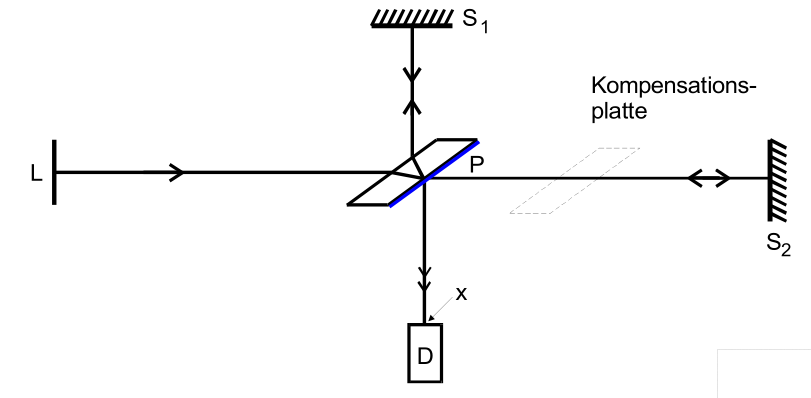
\includegraphics[width = 0.6\textwidth]{content/Interferometer.png}
    \caption{Prinzipieller Aufbau eines Michelson-Interferometers \cite{v401}.}
    \label{fig:Interferometer}
\end{figure}

Eine Komponente ist eine
semipermeable Platte. Eine solche Platte ermöglicht es eine einlaufende Welle aufzuteilen. Dabei wird ein Teil der Welle transmittiert und ein weiterer Teil reflektiert. 
Hierbei bleibt die Wellenlänge jedoch unverändert. Es ändert sich lediglich die Intensität der Welle und bei einem der beiden Strahlen findet an der semipermeablen Platte
ein Phasensprung statt. Diese beiden gespaltenen Wellen werden nun durch den Aufbau überlagert. Da es sich um kohärentes Licht handelt, können die Wellen interferieren. 
Der Gangunterschied der beiden Wellen hängt von der Armlänge des Interferometers ab. Ist ein Arm um $d$ länger als der andere entsteht ein Gangunterschied $w = 2d$.
Daraus kann dann die Intensität der interferierenden Welle durch
\begin{equation*}
    I(d) = 2\text{const}\vec{E}_0^2\left(1 + \cos\left(\frac{2\pi}{\lambda}2d + \pi\right)\right)
\end{equation*}
bestimmt werden. Aus dem Cosinusterm dieser Gleichung kann eine Bedingung für konstruktive und destruktive Interferenz hergeleitet werden. 

Wird nun die Armlänge um einen Wert $\Delta d$ verändert, treten bei einer kontinuierlichen verschiebung abwechselnd Intensitätsmaxima und Minima auf. Aus einer festen 
Verschiebung $\Delta d$ und eine Zählung der Maxima kann über 
\begin{equation}
    \label{eqn:lambda}
    \lambda = \frac{2 \Delta d}{z}
\end{equation}
die Wellenlänge des Strahls berechnet werden. Dabei beschreibt $z$ die Anzahl der detektierten Maxima.

Bei einem Michelson-Interferometer kann ein Gangunterschied allerdings nicht ausschließlich durch eine veränderte Armlänge entstehen. Ebenso kann ein Gangunterschied der Strahlen
durch einen veränderten Brechungsindex in einem der Arme entstehen. Läuft ein Strahl entlang einer Länge $b$ einen Brechungsindex $n + \Delta n$, entsteht dabei
der Gangunterschied $b\Delta n$. Daraus ergibt sich dann über die Maximabedingung der Zusammenhang  
\begin{equation}
    \label{eqn:Delta_n}
    \Delta n = \frac{z\lambda}{2b}.
\end{equation}

\subsection{Abhängikeit des Brechungsindex vom Druck}
\label{subsec:Brechungsindex}
Im folgendem wird angenommen, dass Luft zwischen $\qty{0}{\bar}$ und $\qty{1}{\bar}$ sich wie ein ideales Gas verhält. Aus der idealen Gasgleichung kann die Anzahl der Moleküle
in Abhängikeit vom Druck $p$ und der Temperatur $T$ gemäß 
\begin{equation*}
    N(p,T) = \frac{p}{T}\frac{T_0}{p_0}N_\text{L}
\end{equation*}
berechnet werden. Dabei ist $N_\text{L}$ der die Loschmidtsche Zahl. 
Damit kann nun die Änderung des Brechungsindex durch 
\begin{equation*}
    \Delta n(p,p') = \frac{f}{2}N_\text{L}\frac{T_0}{p_0}\frac{1}{T}(p - p')
\end{equation*}
bestimmt werden.
Wird der Brechungsindex nun unter Normalbedingungen betrachtet, ergibt sich dieser zu 
\begin{equation}
    \label{eqn:Brechungsindex}
    n(p_0, T_0) = 1 + \Delta n(p,p')\frac{T}{T_0}\frac{p_0}{p - p'}.
\end{equation}
